\documentclass[a4paper, 11pt]{article}
\usepackage{comment} % enables the use of multi-line comments (\ifx \fi) 
\usepackage{fullpage} % changes the margin
\usepackage[a4paper, total={7in, 10in}]{geometry}
\usepackage{amsmath,mathtools}
\usepackage{amssymb,amsthm}  % assumes amsmath package installed
\usepackage{float}
\usepackage{graphicx}
\graphicspath{{./images/}}
\usepackage{xcolor}
\usepackage{mdframed}
\usepackage[shortlabels]{enumitem}
\usepackage{indentfirst}
\usepackage{hyperref}
\hypersetup{
	colorlinks=true,
	linkcolor=blue,
	filecolor=magenta,      
	urlcolor=blue!70!red,
	pdftitle={Assignment}, %%%%%%%%%%%%%%%%   WRITE ASSIGNMENT PDF NAME  %%%%%%%%%%%%%%%%%%%%
}
\usepackage[most,many,breakable]{tcolorbox}



\definecolor{mytheorembg}{HTML}{F2F2F9}
\definecolor{mytheoremfr}{HTML}{00007B}


\tcbuselibrary{theorems,skins,hooks}
\newtcbtheorem{problem}{Problem}
{%
	enhanced,
	breakable,
	colback = mytheorembg,
	frame hidden,
	boxrule = 0sp,
	borderline west = {2pt}{0pt}{mytheoremfr},
	sharp corners,
	detach title,
	before upper = \tcbtitle\par\smallskip,
	coltitle = mytheoremfr,
	fonttitle = \bfseries\sffamily,
	description font = \mdseries,
	separator sign none,
	segmentation style={solid, mytheoremfr},
}
{p}

% To give references for any problem use like this
% suppose the problem number is p3 then 2 options either 
% \hyperref[p:p3]{<text you want to use to hyperlink> \ref{p:p3}}
%                  or directly 
%                   \ref{p:p3}



%---------------------------------------
% BlackBoard Math Fonts :-
%---------------------------------------

%Captital Letters
\newcommand{\bbA}{\mathbb{A}}	\newcommand{\bbB}{\mathbb{B}}
\newcommand{\bbC}{\mathbb{C}}	\newcommand{\bbD}{\mathbb{D}}
\newcommand{\bbE}{\mathbb{E}}	\newcommand{\bbF}{\mathbb{F}}
\newcommand{\bbG}{\mathbb{G}}	\newcommand{\bbH}{\mathbb{H}}
\newcommand{\bbI}{\mathbb{I}}	\newcommand{\bbJ}{\mathbb{J}}
\newcommand{\bbK}{\mathbb{K}}	\newcommand{\bbL}{\mathbb{L}}
\newcommand{\bbM}{\mathbb{M}}	\newcommand{\bbN}{\mathbb{N}}
\newcommand{\bbO}{\mathbb{O}}	\newcommand{\bbP}{\mathbb{P}}
\newcommand{\bbQ}{\mathbb{Q}}	\newcommand{\bbR}{\mathbb{R}}
\newcommand{\bbS}{\mathbb{S}}	\newcommand{\bbT}{\mathbb{T}}
\newcommand{\bbU}{\mathbb{U}}	\newcommand{\bbV}{\mathbb{V}}
\newcommand{\bbW}{\mathbb{W}}	\newcommand{\bbX}{\mathbb{X}}
\newcommand{\bbY}{\mathbb{Y}}	\newcommand{\bbZ}{\mathbb{Z}}

%---------------------------------------
% MathCal Fonts :-
%---------------------------------------

%Captital Letters
\newcommand{\mcA}{\mathcal{A}}	\newcommand{\mcB}{\mathcal{B}}
\newcommand{\mcC}{\mathcal{C}}	\newcommand{\mcD}{\mathcal{D}}
\newcommand{\mcE}{\mathcal{E}}	\newcommand{\mcF}{\mathcal{F}}
\newcommand{\mcG}{\mathcal{G}}	\newcommand{\mcH}{\mathcal{H}}
\newcommand{\mcI}{\mathcal{I}}	\newcommand{\mcJ}{\mathcal{J}}
\newcommand{\mcK}{\mathcal{K}}	\newcommand{\mcL}{\mathcal{L}}
\newcommand{\mcM}{\mathcal{M}}	\newcommand{\mcN}{\mathcal{N}}
\newcommand{\mcO}{\mathcal{O}}	\newcommand{\mcP}{\mathcal{P}}
\newcommand{\mcQ}{\mathcal{Q}}	\newcommand{\mcR}{\mathcal{R}}
\newcommand{\mcS}{\mathcal{S}}	\newcommand{\mcT}{\mathcal{T}}
\newcommand{\mcU}{\mathcal{U}}	\newcommand{\mcV}{\mathcal{V}}
\newcommand{\mcW}{\mathcal{W}}	\newcommand{\mcX}{\mathcal{X}}
\newcommand{\mcY}{\mathcal{Y}}	\newcommand{\mcZ}{\mathcal{Z}}



%---------------------------------------
% Bold Math Fonts :-
%---------------------------------------

%Captital Letters
\newcommand{\bmA}{\boldsymbol{A}}	\newcommand{\bmB}{\boldsymbol{B}}
\newcommand{\bmC}{\boldsymbol{C}}	\newcommand{\bmD}{\boldsymbol{D}}
\newcommand{\bmE}{\boldsymbol{E}}	\newcommand{\bmF}{\boldsymbol{F}}
\newcommand{\bmG}{\boldsymbol{G}}	\newcommand{\bmH}{\boldsymbol{H}}
\newcommand{\bmI}{\boldsymbol{I}}	\newcommand{\bmJ}{\boldsymbol{J}}
\newcommand{\bmK}{\boldsymbol{K}}	\newcommand{\bmL}{\boldsymbol{L}}
\newcommand{\bmM}{\boldsymbol{M}}	\newcommand{\bmN}{\boldsymbol{N}}
\newcommand{\bmO}{\boldsymbol{O}}	\newcommand{\bmP}{\boldsymbol{P}}
\newcommand{\bmQ}{\boldsymbol{Q}}	\newcommand{\bmR}{\boldsymbol{R}}
\newcommand{\bmS}{\boldsymbol{S}}	\newcommand{\bmT}{\boldsymbol{T}}
\newcommand{\bmU}{\boldsymbol{U}}	\newcommand{\bmV}{\boldsymbol{V}}
\newcommand{\bmW}{\boldsymbol{W}}	\newcommand{\bmX}{\boldsymbol{X}}
\newcommand{\bmY}{\boldsymbol{Y}}	\newcommand{\bmZ}{\boldsymbol{Z}}
%Small Letters
\newcommand{\bma}{\boldsymbol{a}}	\newcommand{\bmb}{\boldsymbol{b}}
\newcommand{\bmc}{\boldsymbol{c}}	\newcommand{\bmd}{\boldsymbol{d}}
\newcommand{\bme}{\boldsymbol{e}}	\newcommand{\bmf}{\boldsymbol{f}}
\newcommand{\bmg}{\boldsymbol{g}}	\newcommand{\bmh}{\boldsymbol{h}}
\newcommand{\bmi}{\boldsymbol{i}}	\newcommand{\bmj}{\boldsymbol{j}}
\newcommand{\bmk}{\boldsymbol{k}}	\newcommand{\bml}{\boldsymbol{l}}
\newcommand{\bmm}{\boldsymbol{m}}	\newcommand{\bmn}{\boldsymbol{n}}
\newcommand{\bmo}{\boldsymbol{o}}	\newcommand{\bmp}{\boldsymbol{p}}
\newcommand{\bmq}{\boldsymbol{q}}	\newcommand{\bmr}{\boldsymbol{r}}
\newcommand{\bms}{\boldsymbol{s}}	\newcommand{\bmt}{\boldsymbol{t}}
\newcommand{\bmu}{\boldsymbol{u}}	\newcommand{\bmv}{\boldsymbol{v}}
\newcommand{\bmw}{\boldsymbol{w}}	\newcommand{\bmx}{\boldsymbol{x}}
\newcommand{\bmy}{\boldsymbol{y}}	\newcommand{\bmz}{\boldsymbol{z}}

%---------------------------------------
% Scr Math Fonts :-
%---------------------------------------

\newcommand{\sA}{{\mathscr{A}}}   \newcommand{\sB}{{\mathscr{B}}}
\newcommand{\sC}{{\mathscr{C}}}   \newcommand{\sD}{{\mathscr{D}}}
\newcommand{\sE}{{\mathscr{E}}}   \newcommand{\sF}{{\mathscr{F}}}
\newcommand{\sG}{{\mathscr{G}}}   \newcommand{\sH}{{\mathscr{H}}}
\newcommand{\sI}{{\mathscr{I}}}   \newcommand{\sJ}{{\mathscr{J}}}
\newcommand{\sK}{{\mathscr{K}}}   \newcommand{\sL}{{\mathscr{L}}}
\newcommand{\sM}{{\mathscr{M}}}   \newcommand{\sN}{{\mathscr{N}}}
\newcommand{\sO}{{\mathscr{O}}}   \newcommand{\sP}{{\mathscr{P}}}
\newcommand{\sQ}{{\mathscr{Q}}}   \newcommand{\sR}{{\mathscr{R}}}
\newcommand{\sS}{{\mathscr{S}}}   \newcommand{\sT}{{\mathscr{T}}}
\newcommand{\sU}{{\mathscr{U}}}   \newcommand{\sV}{{\mathscr{V}}}
\newcommand{\sW}{{\mathscr{W}}}   \newcommand{\sX}{{\mathscr{X}}}
\newcommand{\sY}{{\mathscr{Y}}}   \newcommand{\sZ}{{\mathscr{Z}}}


%---------------------------------------
% Math Fraktur Font
%---------------------------------------

%Captital Letters
\newcommand{\mfA}{\mathfrak{A}}	\newcommand{\mfB}{\mathfrak{B}}
\newcommand{\mfC}{\mathfrak{C}}	\newcommand{\mfD}{\mathfrak{D}}
\newcommand{\mfE}{\mathfrak{E}}	\newcommand{\mfF}{\mathfrak{F}}
\newcommand{\mfG}{\mathfrak{G}}	\newcommand{\mfH}{\mathfrak{H}}
\newcommand{\mfI}{\mathfrak{I}}	\newcommand{\mfJ}{\mathfrak{J}}
\newcommand{\mfK}{\mathfrak{K}}	\newcommand{\mfL}{\mathfrak{L}}
\newcommand{\mfM}{\mathfrak{M}}	\newcommand{\mfN}{\mathfrak{N}}
\newcommand{\mfO}{\mathfrak{O}}	\newcommand{\mfP}{\mathfrak{P}}
\newcommand{\mfQ}{\mathfrak{Q}}	\newcommand{\mfR}{\mathfrak{R}}
\newcommand{\mfS}{\mathfrak{S}}	\newcommand{\mfT}{\mathfrak{T}}
\newcommand{\mfU}{\mathfrak{U}}	\newcommand{\mfV}{\mathfrak{V}}
\newcommand{\mfW}{\mathfrak{W}}	\newcommand{\mfX}{\mathfrak{X}}
\newcommand{\mfY}{\mathfrak{Y}}	\newcommand{\mfZ}{\mathfrak{Z}}
%Small Letters
\newcommand{\mfa}{\mathfrak{a}}	\newcommand{\mfb}{\mathfrak{b}}
\newcommand{\mfc}{\mathfrak{c}}	\newcommand{\mfd}{\mathfrak{d}}
\newcommand{\mfe}{\mathfrak{e}}	\newcommand{\mff}{\mathfrak{f}}
\newcommand{\mfg}{\mathfrak{g}}	\newcommand{\mfh}{\mathfrak{h}}
\newcommand{\mfi}{\mathfrak{i}}	\newcommand{\mfj}{\mathfrak{j}}
\newcommand{\mfk}{\mathfrak{k}}	\newcommand{\mfl}{\mathfrak{l}}
\newcommand{\mfm}{\mathfrak{m}}	\newcommand{\mfn}{\mathfrak{n}}
\newcommand{\mfo}{\mathfrak{o}}	\newcommand{\mfp}{\mathfrak{p}}
\newcommand{\mfq}{\mathfrak{q}}	\newcommand{\mfr}{\mathfrak{r}}
\newcommand{\mfs}{\mathfrak{s}}	\newcommand{\mft}{\mathfrak{t}}
\newcommand{\mfu}{\mathfrak{u}}	\newcommand{\mfv}{\mathfrak{v}}
\newcommand{\mfw}{\mathfrak{w}}	\newcommand{\mfx}{\mathfrak{x}}
\newcommand{\mfy}{\mathfrak{y}}	\newcommand{\mfz}{\mathfrak{z}}

%---------------------------------------
% Bar
%---------------------------------------

%Captital Letters
\newcommand{\ovA}{\overline{A}}	\newcommand{\ovB}{\overline{B}}
\newcommand{\ovC}{\overline{C}}	\newcommand{\ovD}{\overline{D}}
\newcommand{\ovE}{\overline{E}}	\newcommand{\ovF}{\overline{F}}
\newcommand{\ovG}{\overline{G}}	\newcommand{\ovH}{\overline{H}}
\newcommand{\ovI}{\overline{I}}	\newcommand{\ovJ}{\overline{J}}
\newcommand{\ovK}{\overline{K}}	\newcommand{\ovL}{\overline{L}}
\newcommand{\ovM}{\overline{M}}	\newcommand{\ovN}{\overline{N}}
\newcommand{\ovO}{\overline{O}}	\newcommand{\ovP}{\overline{P}}
\newcommand{\ovQ}{\overline{Q}}	\newcommand{\ovR}{\overline{R}}
\newcommand{\ovS}{\overline{S}}	\newcommand{\ovT}{\overline{T}}
\newcommand{\ovU}{\overline{U}}	\newcommand{\ovV}{\overline{V}}
\newcommand{\ovW}{\overline{W}}	\newcommand{\ovX}{\overline{X}}
\newcommand{\ovY}{\overline{Y}}	\newcommand{\ovZ}{\overline{Z}}
%Small Letters
\newcommand{\ova}{\overline{a}}	\newcommand{\ovb}{\overline{b}}
\newcommand{\ovc}{\overline{c}}	\newcommand{\ovd}{\overline{d}}
\newcommand{\ove}{\overline{e}}	\newcommand{\ovf}{\overline{f}}
\newcommand{\ovg}{\overline{g}}	\newcommand{\ovh}{\overline{h}}
\newcommand{\ovi}{\overline{i}}	\newcommand{\ovj}{\overline{j}}
\newcommand{\ovk}{\overline{k}}	\newcommand{\ovl}{\overline{l}}
\newcommand{\ovm}{\overline{m}}	\newcommand{\ovn}{\overline{n}}
\newcommand{\ovo}{\overline{o}}	\newcommand{\ovp}{\overline{p}}
\newcommand{\ovq}{\overline{q}}	\newcommand{\ovr}{\overline{r}}
\newcommand{\ovs}{\overline{s}}	\newcommand{\ovt}{\overline{t}}
\newcommand{\ovu}{\overline{u}}	\newcommand{\ovv}{\overline{v}}
\newcommand{\ovw}{\overline{w}}	\newcommand{\ovx}{\overline{x}}
\newcommand{\ovy}{\overline{y}}	\newcommand{\ovz}{\overline{z}}

%---------------------------------------
% Tilde
%---------------------------------------

%Captital Letters
\newcommand{\tdA}{\tilde{A}}	\newcommand{\tdB}{\tilde{B}}
\newcommand{\tdC}{\tilde{C}}	\newcommand{\tdD}{\tilde{D}}
\newcommand{\tdE}{\tilde{E}}	\newcommand{\tdF}{\tilde{F}}
\newcommand{\tdG}{\tilde{G}}	\newcommand{\tdH}{\tilde{H}}
\newcommand{\tdI}{\tilde{I}}	\newcommand{\tdJ}{\tilde{J}}
\newcommand{\tdK}{\tilde{K}}	\newcommand{\tdL}{\tilde{L}}
\newcommand{\tdM}{\tilde{M}}	\newcommand{\tdN}{\tilde{N}}
\newcommand{\tdO}{\tilde{O}}	\newcommand{\tdP}{\tilde{P}}
\newcommand{\tdQ}{\tilde{Q}}	\newcommand{\tdR}{\tilde{R}}
\newcommand{\tdS}{\tilde{S}}	\newcommand{\tdT}{\tilde{T}}
\newcommand{\tdU}{\tilde{U}}	\newcommand{\tdV}{\tilde{V}}
\newcommand{\tdW}{\tilde{W}}	\newcommand{\tdX}{\tilde{X}}
\newcommand{\tdY}{\tilde{Y}}	\newcommand{\tdZ}{\tilde{Z}}
%Small Letters
\newcommand{\tda}{\tilde{a}}	\newcommand{\tdb}{\tilde{b}}
\newcommand{\tdc}{\tilde{c}}	\newcommand{\tdd}{\tilde{d}}
\newcommand{\tde}{\tilde{e}}	\newcommand{\tdf}{\tilde{f}}
\newcommand{\tdg}{\tilde{g}}	\newcommand{\tdh}{\tilde{h}}
\newcommand{\tdi}{\tilde{i}}	\newcommand{\tdj}{\tilde{j}}
\newcommand{\tdk}{\tilde{k}}	\newcommand{\tdl}{\tilde{l}}
\newcommand{\tdm}{\tilde{m}}	\newcommand{\tdn}{\tilde{n}}
\newcommand{\tdo}{\tilde{o}}	\newcommand{\tdp}{\tilde{p}}
\newcommand{\tdq}{\tilde{q}}	\newcommand{\tdr}{\tilde{r}}
\newcommand{\tds}{\tilde{s}}	\newcommand{\tdt}{\tilde{t}}
\newcommand{\tdu}{\tilde{u}}	\newcommand{\tdv}{\tilde{v}}
\newcommand{\tdw}{\tilde{w}}	\newcommand{\tdx}{\tilde{x}}
\newcommand{\tdy}{\tilde{y}}	\newcommand{\tdz}{\tilde{z}}

%---------------------------------------
% Vec
%---------------------------------------

%Captital Letters
\newcommand{\vcA}{\vec{A}}	\newcommand{\vcB}{\vec{B}}
\newcommand{\vcC}{\vec{C}}	\newcommand{\vcD}{\vec{D}}
\newcommand{\vcE}{\vec{E}}	\newcommand{\vcF}{\vec{F}}
\newcommand{\vcG}{\vec{G}}	\newcommand{\vcH}{\vec{H}}
\newcommand{\vcI}{\vec{I}}	\newcommand{\vcJ}{\vec{J}}
\newcommand{\vcK}{\vec{K}}	\newcommand{\vcL}{\vec{L}}
\newcommand{\vcM}{\vec{M}}	\newcommand{\vcN}{\vec{N}}
\newcommand{\vcO}{\vec{O}}	\newcommand{\vcP}{\vec{P}}
\newcommand{\vcQ}{\vec{Q}}	\newcommand{\vcR}{\vec{R}}
\newcommand{\vcS}{\vec{S}}	\newcommand{\vcT}{\vec{T}}
\newcommand{\vcU}{\vec{U}}	\newcommand{\vcV}{\vec{V}}
\newcommand{\vcW}{\vec{W}}	\newcommand{\vcX}{\vec{X}}
\newcommand{\vcY}{\vec{Y}}	\newcommand{\vcZ}{\vec{Z}}
%Small Letters
\newcommand{\vca}{\vec{a}}	\newcommand{\vcb}{\vec{b}}
\newcommand{\vcc}{\vec{c}}	\newcommand{\vcd}{\vec{d}}
\newcommand{\vce}{\vec{e}}	\newcommand{\vcf}{\vec{f}}
\newcommand{\vcg}{\vec{g}}	\newcommand{\vch}{\vec{h}}
\newcommand{\vci}{\vec{i}}	\newcommand{\vcj}{\vec{j}}
\newcommand{\vck}{\vec{k}}	\newcommand{\vcl}{\vec{l}}
\newcommand{\vcm}{\vec{m}}	\newcommand{\vcn}{\vec{n}}
\newcommand{\vco}{\vec{o}}	\newcommand{\vcp}{\vec{p}}
\newcommand{\vcq}{\vec{q}}	\newcommand{\vcr}{\vec{r}}
\newcommand{\vcs}{\vec{s}}	\newcommand{\vct}{\vec{t}}
\newcommand{\vcu}{\vec{u}}	\newcommand{\vcv}{\vec{v}}
\newcommand{\vcw}{\vec{w}}	\newcommand{\vcx}{\vec{x}}
\newcommand{\vcy}{\vec{y}}	\newcommand{\vcz}{\vec{z}}

%---------------------------------------
% Greek Letters:-
%---------------------------------------
\newcommand{\eps}{\epsilon}
\newcommand{\veps}{\varepsilon}
\newcommand{\lm}{\lambda}
\newcommand{\Lm}{\Lambda}
\newcommand{\gm}{\gamma}
\newcommand{\Gm}{\Gamma}
\newcommand{\vph}{\varphi}
\newcommand{\ph}{\phi}
\newcommand{\om}{\omega}
\newcommand{\Om}{\Omega}


%%%%%%%%%%%%%%%%%%%%%%%%%%%%%%%%%%%%%%%% MACROS %%%%%%%%%%%%%%%%%%%%%%%%%%%%%%%%%%%%%%%%

%%%%%%%%%%%%%%% Link With an Icon %%%%%%%%%%%%%%% 
\newcommand{\link}[1]{
    \href{#1}{\faIcon{link}}
}

%%%%%%%%%%%%%%% Name Template %%%%%%%%%%%%%%% 
\newcommand{\name}[2]{
    % Name
    \Huge % Font size
    \raggedright \textbf{#1} \par

    \vspace*{0.3cm}
    
    % Profession
    \Large % Font size
    \raggedright #2 \par
    \normalsize \normalfont
}

%%%%%%%%%%%%%%% Contact Details %%%%%%%%%%%%%%%
\newcommand{\info}[2]{
    \faIcon{#2} \hspace{0.2em} #1
}

%%%%%%%%%%%%%%% Email %%%%%%%%%%%%%%%
\newcommand{\email}[1]{
    \info{#1}{envelope}
}

%%%%%%%%%%%%%%% Phone Number %%%%%%%%%%%%%%%
\newcommand{\phone}[1]{
    \info{#1}{mobile-alt}
}

%%%%%%%%%%%%%%% Address %%%%%%%%%%%%%%%
\newcommand{\address}[1]{
    \info{#1}{map-marker-alt}
}

%%%%%%%%%%%%%%% GitHub %%%%%%%%%%%%%%%
\newcommand{\github}[2]{
    \info{\href{#1}{\underline{#2}}}{github}
}

%%%%%%%%%%%%%%% LinkedIn %%%%%%%%%%%%%%%
\newcommand{\linkedin}[2]{
    \info{\href{#1}{\underline{#2}}}{linkedin}
}

%%%%%%%%%%%%%%% ResearchGate %%%%%%%%%%%%%%%
\newcommand{\researchgate}[2]{
    \info{\href{#1}{\underline{#2}}}{researchgate}
}

%%%\newcommand*{\Researchgate}[1]{\sociallink{\researchgatesocialsymbol}{http://www.#1}{#1}}

%%%%%%%%%%%%%%% Website %%%%%%%%%%%%%%%
\newcommand{\website}[1]{
    \info{#1}{link}
}

%%%%%%%%%%%%%%% Draw Skill Bars %%%%%%%%%%%%%%% 
\newcommand{\drawskillbars}[1]{
    \begin{tikzpicture}
        % Draw 5 gray bars
        \foreach \i in {0, 1, 2, 3, 4}{
            \fill[lightgray] (\i * 0.7 + 0.2 *\i,0) rectangle (0.7 + \i * 0.7 + \i * 0.2,0.1);
        }
        
        % Draw number of black bars depending on the skill level
        \foreach \i in {#1}{
            \fill[blue!40] (\i * 0.7 + 0.2 *\i,0) rectangle (0.7 + \i * 0.7 + \i * 0.2,0.1);
            %\fill[title] (\i * 0.7 + 0.2 *\i,0) rectangle (0.7 + \i * 0.7 + \i * 0.2,0.1);
        }
    \end{tikzpicture} \par
}
    
%%%%%%%%%%%%%%% Skills %%%%%%%%%%%%%%%
\newcommand{\skill}[3]{
    % Name of the skill
    \large
    \noindent \hangafter=0
    \adjustbox{valign=t}{\begin{minipage}{0.72\textwidth}
        \large \noindent \hangafter=0
        % Name of the skill
        \textmd{#1} 
        \normalsize \par 
        \vspace{1em}
         % Description
        \noindent \small \color{subtitle} \parbox{1\linewidth}{\textsl{#3}} \par
        \normalsize \par
        \end{minipage}}
    \adjustbox{valign=t}{\begin{minipage}{0.2\textwidth}
        % Skill bars
        \large \hangafter=0
        %\noindent 
        \drawskillbars{#2}
        \end{minipage}}
    \normalsize \par 
    % Skill bars
    %%\drawskillbars{#2}
    %%\vspace{0.5em}
    
    \vspace{1.0em}
    \normalsize \color{black} \par
}

%%%%%%%%%%%%%%% Software %%%%%%%%%%%%%%%
\newcommand{\soft}[2]{
    \adjustbox{valign=t}{\begin{minipage}{0.40\textwidth}
        \large \noindent \hangafter=0
        % Name of the skill
        \textmd{#1} 
        \normalsize \par 
        \vspace{1em}
        \end{minipage}}
    \adjustbox{valign=t}{\begin{minipage}{0.5\textwidth}
        % Skill bars
        \large \noindent \hangafter=0
        \drawskillbars{#2}
        \end{minipage}}
    \normalsize \par 
    \vspace{1em}
}

%%%%%%%%%%%%%%% Personal details %%%%%%%%%%%%%%%
\newcommand{\details}[2]{
    % Name of the language
    \large
    \noindent \hangafter=0 \color{black}
    \adjustbox{valign=t}{\parbox{0.27\linewidth}{#1}}  \adjustbox{valign=t}{\parbox{0.55\linewidth}{#2}} \par
    \vspace{.3em}
    \normalsize \color{black} \par
 }

%%%%%%%%%%%%%%% Language %%%%%%%%%%%%%%%
\newcommand{\lan}[2]{
    % Name of the language
    \large
    \noindent \hangafter=0 \color{black}
    \parbox{0.3\linewidth}{\textmd{#1}}   \color{subtitle} \parbox{0.4\linewidth}{\textsl{#2}} \par
    %\large English \color{subtitle} \textit{Advanced} 
    %\normalsize \par 
    % Knowledge level
    %\noindent \small \color{subtitle} \parbox{1\linewidth}{\textsl{#2}} \par
    \vspace{1.0em}
    \normalsize \color{black} \par
 }

%%%%%%%%%%%%%%% Education %%%%%%%%%%%%%%%
\newcommand{\education}[4]{
    % Name of the studies
    \noindent \large \parbox{.65\linewidth}{\textbf{#1}}
    % Duration in a Box
    \hfill \small
    \tcbox[enhanced,nobeforeafter,box align=base,colback=title,colframe=title,size=fbox,arc=0mm, valign=bottom]{{\textbf{#2}}} \par
    \vspace{0.3em}
    % School Name 
    \normalsize
    \noindent \color{subtitle} \parbox{.9\linewidth}{\textsl{#3}} \par
    % Description
    \normalsize \color{black}
    \vspace*{0.3em}
    \small #4 
    \normalsize \par
    \vspace*{0.5em}
}

%%%%%%%%%%%%%%% Work Experience %%%%%%%%%%%%%%%
\newcommand{\work}[4]{
    % Name of the Job
    \noindent \large \parbox{.65\linewidth}{\textbf{#1}}
    % Duration in a Box 
    \hfill \small
    \tcbox[enhanced,box align=base,nobeforeafter,colback=title,colframe=title,size=fbox,arc=0mm]{\textbf{#2}} \par
    \vspace{0.3em}
    % Name of the Employer
    \noindent \large \color{subtitle} \parbox{.9\linewidth}{\textsl{#3}} \par
    % Description of the job
    \vspace*{0.3em} \color{black}
    \small #4 
    \normalsize \par
}

%%%%%%%%%%%%%%% Teaching %%%%%%%%%%%%%%%
\newcommand{\teaching}[3]{
    % What, Topic and Who/Where/when
    \noindent \adjustbox{valign=t}{\parbox{.99\linewidth}{\text{#1} \text{#2} \textbf{#3}}} 
    \vspace{0.5em}
    \vspace*{1em} 
}

%%%%%%%%%%%%%%% Publications %%%%%%%%%%%%%%%
\newcommand{\publ}[4]{
    % Authors, Title and journal
    \noindent \parbox{.99\linewidth}{\textsl{#3}. \textbf{#1} \textsl{#2} \link{#4}}
    \vspace{0.5em}
    \vspace*{1em} \color{black}
    }

%%%%%%%%%%%%%%% Talks %%%%%%%%%%%%%%%
\newcommand{\talk}[3]{
    % Authors, Title and journal
    \noindent \parbox{.99\linewidth}{\textsl{#3}. \textbf{#1} \textsl{#2}}
    \vspace{0.5em}
    \vspace*{1em} \color{black}
}

%%%%%%%%%%%%%%% Events %%%%%%%%%%%%%%%
\newcommand{\event}[3]{
    \noindent \parbox{.99\linewidth}{\textbf{#1} \textsl{#3} \textsl{#2}}
    \vspace{0.5em}
    \vspace*{1em} \color{black}
}

\setlength{\parindent}{0pt}

%%%%%%%%%%%%%%%%%%%%%%%%%%%%%%%%%%%%%%%%%%%%%%%%%%%%%%%%%%%%%%%%%%%%%%%%%%%%%%%%%%%%%%%%%%%%%%%%%%%%%%%%%%%%%%%%%%%%%%%%%%%%%%%%%%%%%%%%

\begin{document}
	
	%%%%%%%%%%%%%%%%%%%%%%%%%%%%%%%%%%%%%%%%%%%%%%%%%%%%%%%%%%%%%%%%%%%%%%%%%%%%%%%%%%%%%%%%%%%%%%%%%%%%%%%%%%%%%%%%%%%%%%%%%%%%%%%%%%%%%%%%
	
	\textsf{\noindent \large\textbf{Soham Chatterjee} \hfill \textbf{Assignment - 3}\\
		Email: \href{sohamc@cmi.ac.in}{sohamc@cmi.ac.in} \hfill Roll: BMC202175\\
		\normalsize Course: Complex Analysis \hfill Date: March 8, 2023}
	
	%%%%%%%%%%%%%%%%%%%%%%%%%%%%%%%%%%%%%%%%%%%%%%%%%%%%%%%%%%%%%%%%%%%%%%%%%%%%%%%%%%%%%%%%%%%%%%%%%%%%%%%%%%%%%%%%%%%%%%%%%%%%%%%%%%%%%%%%
	% Problem 1
	%%%%%%%%%%%%%%%%%%%%%%%%%%%%%%%%%%%%%%%%%%%%%%%%%%%%%%%%%%%%%%%%%%%%%%%%%%%%%%%%%%%%%%%%%%%%%%%%%%%%%%%%%%%%%%%%%%%%%%%%%%%%%%%%%%%%%%%%
	
	\begin{problem}{%problem statement
			Ahlfors Page 96: Problem 1
		}{p1% problem reference text
		}
		Map the common part of the disks $|z|<1$ and $|z-1|<1$ on the inside of the unit circle. Choose the mapping so that the two symmetries are preserved.
		%Problem		
	\end{problem}
	
	\solve{
		%Solution
		\begin{center}
			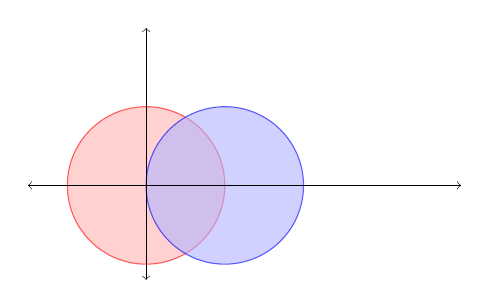
\begin{tikzpicture}
				\filldraw[red!30!white,opacity=0.6,draw=red] (0,0) circle (1cm);
				\filldraw[blue!30!white,opacity=0.6,draw=blue] (1,0) circle (1cm);
				\draw[<->,very thin] (-1.5,0) -- (4,0);
				\draw[<->,very thin] (0,-1.2) -- (0,2);
			\end{tikzpicture}
		\end{center}
		
		
	}
	
	
	%%%%%%%%%%%%%%%%%%%%%%%%%%%%%%%%%%%%%%%%%%%%%%%%%%%%%%%%%%%%%%%%%%%%%%%%%
	% Problem 2
	%%%%%%%%%%%%%%%%%%%%%%%%%%%%%%%%%%%%%%%%%%%%%%%%%%%%%%%%%%%%%%%%%%%%%%%%%
	
	\begin{problem}{%problem statement
			Ahlfors Page 96: Problem 2
		}{p2% problem reference text
		}
		%Problem		
			Map the region between $|z|=1$ and $\left|z-\frac{1}{2}\right|=\frac{1}{2}$ on a half plane.
		
	\end{problem}                               
	
	\solve{
		%Solution
	
	}
	
	
	%%%%%%%%%%%%%%%%%%%%%%%%%%%%%%%%%%%%%%%%%%%%%%%%%%%%%%%%%%%%%%%%%%%%%%%%%
	% Problem 3
	%%%%%%%%%%%%%%%%%%%%%%%%%%%%%%%%%%%%%%%%%%%%%%%%%%%%%%%%%%%%%%%%%%%%%%%%%
	
	\begin{problem}{%problem statement
			Ahlfors Page 97: Problem 3
		}{p3% problem reference text
		}
		%Problem
		Map the complement of the arc $|z|=1$, $y\geq 0$ on the outside of the unit circle so that the points at  $\infty$ correspond to each other
	\end{problem}
	
	\solve{
		%Solution

	}
	
	
	%%%%%%%%%%%%%%%%%%%%%%%%%%%%%%%%%%%%%%%%%%%%%%%%%%%%%%%%%%%%%%%%%%%%%%%%%
	% Problem 4
	%%%%%%%%%%%%%%%%%%%%%%%%%%%%%%%%%%%%%%%%%%%%%%%%%%%%%%%%%%%%%%%%%%%%%%%%%
	
	\begin{problem}{%problem statement
			Ahlfors Page 108: Problem 1
		}{p4% problem reference text
		}
		%Problem		
Compute
$$
\int_\gamma x d z
$$
where $\gamma$ is the directed line segment from 0 to $1+i$.
	\end{problem}
	
	\solve{
		%Solution
		
		$\gm$ is the directed line segment from $0$ to $1+i$. Hence  $z=t(1+i)$ where $t\in[0,1]$. Then we have $$dz=(1+i)dt$$then \begin{align*}
			\int_{\gm} xdz & = \int_0^1\Re(t(1+i))(1+i)dt      \\
			               & = \int_0^1 t(1+i)dt               \\
			               & = (1+i)\int_0^1tdt                \\
			               & = (1+i)\lt[ \frac{t^2}{2}\rt]_0^1 \\
			               & = \frac{1+i}{2}
		\end{align*}
	}
	

	%%%%%%%%%%%%%%%%%%%%%%%%%%%%%%%%%%%%%%%%%%%%%%%%%%%%%%%%%%%%%%%%%%%%%%%%%
	% Problem 5
	%%%%%%%%%%%%%%%%%%%%%%%%%%%%%%%%%%%%%%%%%%%%%%%%%%%%%%%%%%%%%%%%%%%%%%%%%
	
	\begin{problem}{%problem statement
Ahlfors Page 108: Problem 2
		}{p5% problem reference text
		}
		%Problem		
	Compute
	$$
	\int_{|z|=r} x d z
	$$
	for the positive sense of the circle, in two ways: first, by use of a parameter, and second, by observing that $x=\frac{1}{2}(z+\bar{z})=\frac{1}{2}\left(z+\frac{r^2}{z}\right)$ on the circle.
	\end{problem}
	
	\solve{
		%Solution
		\begin{itemize}
			\item Given that $|z|=r$. Therefore $z=re^{i\theta}$ where $\theta\in [0,2\pi]$. Hence $$dz=ire^{i\theta}d\theta$$\begin{align*}
				\int_{|z|=r} x d z & = \int_0^{2\pi} \Re(re^{i\theta})\lt(ire^{i\theta}d\theta\rt)\\
				& =\int_0^{2\pi} \Re(r\lt(\cos\theta +i\sin\theta\rt))\lt(ir\lt(\cos\theta+i\sin\theta\rt)\rt)d\theta\\
				&= ir^2\int_0^{2\pi} \cos\theta \lt(\cos\theta+i\sin\theta\rt)d\theta\\
				&=ir^2\lt[\int_0^{2\pi}\cos^2\theta d\theta +i\int_0^{2\pi}\cos\theta\sin\theta d\theta \rt]\\
				&=ir^2\lt[\frac12\int_0^{2\pi}(\cos2\theta+1)d\theta+\frac{i}2\int_0^{2\pi}\sin2\theta d\theta \rt]\\
				&=ir^2\lt[\frac12 \int_0^{2\pi}d\theta\rt]\\
				&=ir^2\frac12(2\pi-0)\\
				&=i\pi r^2
			\end{align*}
		\item \begin{align*}
				\int_{|z|=r} x d z & = 	\int_{|z|=r}\frac{1}{2}(z+\bar{z})dz=	\int_{|z|=r}\frac{1}{2}\left(z+\frac{r^2}{z}\right)dz\\
				& = 	\underbrace{\frac12\int_{|z|=r}zdz}_{\substack{=0\\ \text{As }f\text{ is analytic}}}	+\frac{r^2}2\int_{|z|=r}\frac1zdz\\
				& = \frac{r^2}{2}2\pi i=i\pi r^2
		\end{align*}
		\end{itemize}
		}
	
		%%%%%%%%%%%%%%%%%%%%%%%%%%%%%%%%%%%%%%%%%%%%%%%%%%%%%%%%%%%%%%%%%%%%%%%%%
	% Problem 6
	%%%%%%%%%%%%%%%%%%%%%%%%%%%%%%%%%%%%%%%%%%%%%%%%%%%%%%%%%%%%%%%%%%%%%%%%%
	
	\begin{problem}{%problem statement
			Ahlfors Page 108: Problem 3
		}{p5% problem reference text
		}
		%Problem		
Compute
$$
\int_{|z|=2} \frac{d z}{z^2-1}
$$
for the positive sense of the circle.
	\end{problem}
	
	\solve{
		%Solution
		Given that $|z|=2$. \begin{align*}
			\int_{|z|=2}\frac{dz}{z^2-1} & =\frac12\int_{|z|=2}\frac{(z+1)-(z-1)}{z^2-1}dz\\
			& = \frac12\int_{|z|=2} \lt[ \frac1{z-1}-\frac1{z+1}\rt]dz\\
			& =\frac12\lt[ \int_{|z|=2}\frac{dz}{z-1}-\int_{|z|=2}\frac{dz}{z+1}\rt]\\
			&=\frac12[2\pi i-2\pi i]=0
		\end{align*}
		
	}
		%%%%%%%%%%%%%%%%%%%%%%%%%%%%%%%%%%%%%%%%%%%%%%%%%%%%%%%%%%%%%%%%%%%%%%%%%
	% Problem 7
	%%%%%%%%%%%%%%%%%%%%%%%%%%%%%%%%%%%%%%%%%%%%%%%%%%%%%%%%%%%%%%%%%%%%%%%%%
	
	\begin{problem}{%problem statement
			Ahlfors Page 118: Problem 3
		}{p5% problem reference text
		}
		%Problem
	\parinn The \textit{Jordan curve theorem} asserts that every Jordan curve in the plane determines exactly two regions. The notion of winding number leads to a quick proof of one part of the theorem, namely that the complement of a Jordan curve $\gamma$ has at least two components. This will be so if there exists a point $a$ with $n(\gamma, a) \neq 0$.
	
	We may assume that $\Re (z)>0$ on $\gamma$, and that there are points $z_1$, $z_2 \in \gamma$ with $\Im (z_1)<0, \Im (z)_2>0$. These points may be chosen so that there are no other points of $\gamma$ on the line segments from 0 to $z_1$ and from 0 to $z_2$. Let $\gamma_1$ and $\gamma_2$ be the ares of $\gamma$ from $z_1$ to $z_2$ (excluding the end points).
	
	Let $\sigma_1$ be the closed curve that consists of the line segment from 0 to $z_1$ followed by $\gamma_1$ and the segment from $z_2$ to 0 , and let $\sigma_2$ be constructed in the same way with $\gamma_2$ in the place of $\gamma_1$. Then $\sigma_1-\sigma_2=\gamma$ or $-\gamma$. 
	
	The positive real axis intersects both $\gamma_1$ and $\gamma_2$ (why?). Choose the notation so that the intersection $x_2$ farthest to the right is with $\gamma_2$ (Figure). Prove the following:
	\begin{enumerate}[label=(\alph*)]
		\item $n\left(\sigma_1, x_2\right)=0$, hence $n\left(\sigma_1, z\right)=0$ for $z \epsilon \gamma_2$;
		\item $n\left(\sigma_1, x\right)=n\left(\sigma_2, x\right)=1$ for small $x>0$ (Lemma 2);
		\item the first intersection $x_1$ of the positive real axis with $\gamma$ lies on $\gamma_1$;
		\item $n\left(\sigma_2, x_1\right)=1$, hence $n\left(\sigma_2, z\right)=1$ for $z \epsilon \gamma_1$;
		\item there exists a segment of the positive real axis with one end point on $\gamma_1$, the other on $\gamma_2$, and no other points on $\gamma$. The points $x$ between the end points satisfy $n(\gamma, x)=1$ or -1 .
		
	\end{enumerate}
\begin{center}
	\begin{minipage}[t]{0.5\linewidth}
		\centering
		\includegraphics[width=8cm]{jct.png}
	\end{minipage}
\end{center}
	\end{problem}
	
	\solve{
		%Solution
	
	}

	
		%%%%%%%%%%%%%%%%%%%%%%%%%%%%%%%%%%%%%%%%%%%%%%%%%%%%%%%%%%%%%%%%%%%%%%%%%
	% Problem 8
	%%%%%%%%%%%%%%%%%%%%%%%%%%%%%%%%%%%%%%%%%%%%%%%%%%%%%%%%%%%%%%%%%%%%%%%%%
	
	\begin{problem}{%problem statement
			Ahlfors Page 120: Problem 1
		}{p5% problem reference text
		}
		%Problem		
	Compute
	$$
	\int_{|z|=1} \frac{e^z}{z} d z
	$$
	\end{problem}
	
	\solve{
		%Solution
	$f(z)=e^z$ is analytic on $\bbC$. By Cauchy's Integral Formula we have $$f(z)=\frac{1}{2\pi i}\int_{|\zeta|=1}\frac{f(\zeta)d\zeta}{\zeta-z}=\frac{1}{2\pi i}\int_{|\zeta|=1}\frac{e^{\zeta}d\zeta}{\zeta-z}$$Hence $$1=e^0=f(0)=\frac1{2\pi i}\int_{|\zeta|=1}\frac{e^{\zeta}}{\zeta}d\zeta \iff \int_{|z|=1}\frac{e^z}{z}dz=2\pi i$$
	}
		%%%%%%%%%%%%%%%%%%%%%%%%%%%%%%%%%%%%%%%%%%%%%%%%%%%%%%%%%%%%%%%%%%%%%%%%%
	% Problem 9
	%%%%%%%%%%%%%%%%%%%%%%%%%%%%%%%%%%%%%%%%%%%%%%%%%%%%%%%%%%%%%%%%%%%%%%%%%
	\begin{problem}{%problem statement
			Ahlfors Page 120: Problem 2
		}{p5% problem reference text
		}
		%Problem		
		Compute
		$$
		\int_{|z|=2} \frac{d z}{z^2+1}
		$$
		by decomposition of the integrand in partial fractions.

	\end{problem}
	
	\solve{
		%Solution
		\begin{align*}
			\int_{|z|=2} \frac{d z}{z^2+1} & =\frac1{2i}	\int_{|z|=2}\frac{(z+i)-(z-i)}{(z+i)(z-i)}dz\\
			&= \frac1{2i}	\int_{|z|=2}\lt[ \frac{1}{z-i}-\frac1{z+i}\rt]dz\\
			& = \frac1{2i}\lt[ 	\int_{|z|=2}\frac1{z-i}dz-	\int_{|z|=2}\frac{1}{z+i}dz \rt]\\
			& = \frac1{2i}[2\pi i-2\pi i]=0
		\end{align*}
	 	}
		
	%%%%%%%%%%%%%%%%%%%%%%%%%%%%%%%%%%%%%%%%%%%%%%%%%%%%%%%%%%%%%%%%%%%%%%%%%
	% Problem 10
	%%%%%%%%%%%%%%%%%%%%%%%%%%%%%%%%%%%%%%%%%%%%%%%%%%%%%%%%%%%%%%%%%%%%%%%%%
	
	\begin{problem}{%problem statement
			Ahlfors Page 120: Problem 3
				}{p5% problem reference text
		}
		%Problem		
	Compute
	$$
	\int_{|z|=\rho} \frac{|d z|}{|z-a|^2}
	$$
	under the condition $|a| \neq \rho$. Hint: make use of the equations $z \bar{z}=\rho^2$ and
	$$
	|d z|=-i \rho \frac{d z}{z} .
	$$
		
	\end{problem}
	
	\solve{
		%Solution
		We have $|dz|=-i\rho \frac{dz}{z}$. Therefore \begin{align*}
			\int_{|z|=\rho}\frac{|dz|}{|z-a|^2} & = -i\rho \int_{|z|=\rho}\frac{dz}{z|z-a|^2}= -i\rho \int_{|z|=\rho}\frac{dz}{z(z-a)(\ovz-\ova)}\\
			& = -i\rho \int_{|z|=\rho}\frac{dz}{(z-a)\lt(z\ovz-\ova z  \rt)}\\
			& = -i\rho \int_{|z|=\rho}\frac{dz}{(z-a)\lt(\frac{\rho^2}{z}z-\ova z\rt)}\\
			& = -i\rho \int_{|z|=\rho}\frac{dz}{(z-a)\lt(\rho^2-\ova z\rt)}
		\end{align*}
	
	Now if $\rho < |a|$, then $|z-a|^2>0$. Hence the function $\frac1{(z-a)\lt(\rho^2-\ova z\rt)}$ is analytic and its integral  along $|z|=\rho$ is 0
	
	If $\rho > |a|$ then if $\rho^2\neq \ova z$ because if it is then \begin{align*}
		\rho^2\neq \ova z \iff |z| =\frac{\rho^2}{|a|} \iff \rho = \frac{\rho^2}{|a|} \iff |a|=\rho
	\end{align*} which is not possible. Hence $f(z)=\frac{1}{\rho^2-\ova z}$ is analytic in the $\rho$-disk. Hence $$\int_{|z|=\rho}\frac{dz}{\rho^2-\ova z}=0$$. Then by Cauchy's Integral Formula we have $$f(a)=\frac1{2\pi i}\int_{|z|=\rho}\frac{f(z)dz}{z-a}=\frac{1}{2\pi i}\int_{|z|=\rho}\frac{dz}{(z-a)\lt(\rho^2-\ova z\rt)} \iff $$ Therefore we have $$\int_{|z|=\rho}\frac{|dz|}{|z-a|^2} =-i\rho f(a)2\pi i=-i\rho \frac{2\pi i}{\rho^2-a\ova}=\frac{2\pi \rho}{\rho^2-a\ova}$$
	}
	%%%%%%%%%%%%%%%%%%%%%%%%%%%%%%%%%%%%%%%%%%%%%%%%%%%%%%%%%%%%%%%%%%%%%%%%%
	% Problem 11
	%%%%%%%%%%%%%%%%%%%%%%%%%%%%%%%%%%%%%%%%%%%%%%%%%%%%%%%%%%%%%%%%%%%%%%%%%
	
	\begin{problem}{%problem statement
			Ahlfors Page 123: Problem 1
		}{p5% problem reference text
		}
		%Problem		
		Compute
		$$
		\int_{|z|=1} e^z z^{-n} d z, \quad \int_{|z|=2} z^n(1-z)^m d z, \quad \int_{|z|=\rho}|z-a|^{-4}|d z|(|a| \neq \rho) .
		$$		
	\end{problem}
	
	\solve{
		%Solution
	\begin{itemize}
		\item Let $f(z)e^z$ Then we have $$e^z=f^{((n-1))}(z)=\frac{(n-1)!}{2\pi i}\int_{|\zeta|=1}\frac{f(\zeta)d\zeta}{(\zeta-z)^{n}}=\frac{(n-1)!}{2\pi i}\int_{|\zeta|=1}\frac{e^{\zeta}d\zeta}{(\zeta-z)^{n}}$$Therefore 
			$$f(0)=e^0=1=\frac{(n-1)!}{2\pi i}\int_{|\zeta|=1}\frac{e^z}{z^{n}}dz\iff \int_{|\zeta|=1}\frac{e^z}{z^{n}}dz=\frac{2\pi i}{(n-1)!}$$
		\item 
		\item 
	\end{itemize}
	}
		
	%%%%%%%%%%%%%%%%%%%%%%%%%%%%%%%%%%%%%%%%%%%%%%%%%%%%%%%%%%%%%%%%%%%%%%%%%
	% Problem 12
	%%%%%%%%%%%%%%%%%%%%%%%%%%%%%%%%%%%%%%%%%%%%%%%%%%%%%%%%%%%%%%%%%%%%%%%%%
	
	\begin{problem}{%problem statement
			Ahlfors Page 123: Problem 2
		}{p5% problem reference text
		}
		%Problem		
		Prove that a function which is analytic in the whole plane and satisfies an inequality $|f(z)|<|z|^n$ for some $n$ and all sufficiently large $|z|$ reduces to a polynomial.
		
	\end{problem}
	
	\solve{
		%Solution
		
}
	
	%%%%%%%%%%%%%%%%%%%%%%%%%%%%%%%%%%%%%%%%%%%%%%%%%%%%%%%%%%%%%%%%%%%%%%%%%
	% Problem 13
	%%%%%%%%%%%%%%%%%%%%%%%%%%%%%%%%%%%%%%%%%%%%%%%%%%%%%%%%%%%%%%%%%%%%%%%%%

\begin{problem}{%problem statement
		Ahlfors Page 123: Problem 3
	}{p5% problem reference text
	}
	%Problem		
If $f(z)$ is analytic and $|f(z)| \leqq M$ for $|z| \leqq R$, find an upper bound for $\left|f^{(n)}(z)\right|$ in $|z| \leqq \rho<R$.
	
\end{problem}

\solve{
	%Solution
	
}

	%%%%%%%%%%%%%%%%%%%%%%%%%%%%%%%%%%%%%%%%%%%%%%%%%%%%%%%%%%%%%%%%%%%%%%%%%
	% Problem 14
	%%%%%%%%%%%%%%%%%%%%%%%%%%%%%%%%%%%%%%%%%%%%%%%%%%%%%%%%%%%%%%%%%%%%%%%%%

\begin{problem}{%problem statement
		Ahlfors Page 123: Problem 4
	}{p5% problem reference text
	}
	%Problem		
		If $f(z)$ is analytic for $|z|<1$ and $|f(z)| \leqq 1 /(1-|z|)$, find the best estimate of $\left|f^{(n)}(0)\right|$ that Cauchy's inequality will yield.
	
\end{problem}

\solve{
	%Solution
		We have $$f^{(n)}(z)=\frac{n!}{2\pi i}\int_{|s|=\rho}\frac{f(s)ds}{(s-z)^{n+1}}$$
	\parinf
	\textbf{\textit{Claim: }}$\lt|f^{(n)}(z)\rt|\leq (n+1)!e$
	
	\textbf{\textit{Proof: }}Let for any $k\in \bbN$, $|z|= 1-\frac1k=r_k$. Then $$|f(z)|\leq \frac{1}{1-|z|}=\frac1{1-\frac1k}=k$$Then we have $$\lt|f^{(n)}(0)\rt|=\lt|\frac{n!}{2\pi }\int_{|z|=r_k}\frac{f(z)dz}{z^{n+1}}  \rt|\leq \frac{n!}{2\pi }\int_{|z|=r_k}\frac{|f(z)|}{|z|^{n+1}}|dz|\leq\frac{n!}{2\pi }\, \frac{k}{r_k^{n+1}}2\pi r_k=\frac{kn!}{\lt(1-\frac1k\rt)^{n+1}}=\frac{n!k^{n+2}}{(k-1)^{n+1}}$$Now taking $k=n+1$ we have $$\lt|f^{(n)}(0)\rt|\leq \frac{n!(n+1)^{n+2}}{n^{n+1}} =(n+1)!\frac{(n+1)^{n+1}}{n^{n+1}}=(n+1)!\lt(1+\frac1n\rt)^{n+1}\leq (n+1)!e$$
	
	\parinn
	
	Hence we have the best estimate of $\lt|f^{(n)}(0)\rt|$ which is $\lt|f^{(n)}(0)\rt|\leq (n+1)!e$
	
}


	%%%%%%%%%%%%%%%%%%%%%%%%%%%%%%%%%%%%%%%%%%%%%%%%%%%%%%%%%%%%%%%%%%%%%%%%%
	% Problem 15
	%%%%%%%%%%%%%%%%%%%%%%%%%%%%%%%%%%%%%%%%%%%%%%%%%%%%%%%%%%%%%%%%%%%%%%%%%

\begin{problem}{%problem statement
		Ahlfors Page 123: Problem 5
	}{p5% problem reference text
	}
	%Problem		
		Show that the successive derivatives of an analytic function at a point can never satisfy $\left|f^{(n)}(z)\right|>n ! n^n$. Formulate a sharper theorem of the same kind.
	
\end{problem}

\solve{
	%Solution
	We have $$f^{(n)}(z)=\frac{n!}{2\pi i}\int_{|s|=\rho}\frac{f(s)ds}{(s-z)^{n+1}}$$Hence $$\lt|f^{(n)}(z)\rt|=\lt|\frac{n!}{2\pi i}\int_{|s|=\rho}\frac{f(s)ds}{(s-z)^{n+1}}  \rt|\leq \frac{n!}{2\pi}\int_{|s|=\rho}\lt|\frac{f(s)ds}{(s-z)^{n+1}}\rt|=\frac{n!}{2\pi}\int_{|s|=\rho}\frac{|f(s)|}{|s-z|^{n+1}}|ds|$$Since $f$ is continuous in the $\rho$-disk it is bounded by some value $M$. Therefore$$\lt|f^{(n)}(z)\rt|\leq \frac{n!}{2\pi}\int_{|s|=\rho}\frac{|f(s)|}{|s-z|^{n+1}}|ds|\leq \frac{n!}{2\pi}\int_{|s|=\rho}\frac{M}{|s-z|^{n+1}}|ds|\leq \frac{Mn!}{2\pi}\frac{1}{|\rho-z|^{n+1}}2\pi\rho=Mn!\frac{\rho}{|\rho-z|^{n+1}}$$Since $\rho>|z|$ we have $$\lt|f^{(n)}(z)\rt|\leq Mn!\frac{\rho}{|\rho-z|^{n+1}}\leq Mn!\frac{\rho}{(|\rho|-|z|)^{n+1}}\leq Mn!\frac{\rho}{(|\rho|)^{n+1}}=\frac{Mn!}{\rho^n}$$ Using the given inequality we have $$n!n^n<\lt|f^{(n)}(z)\rt|\leq \frac{Mn!}{\rho^n} \iff n!n^n<\frac{Mn!}{\rho^n}\iff (n\rho )^n<M$$ which is not possible as $n\to \infty$. Hence $f$ doesn't satisfy $\left|f^{(n)}(z)\right|>n ! n^n$
}

	
\end{document}
